\documentclass{article}
\usepackage[utf8]{inputenc}
\usepackage[margin = 1.1in, headheight = 0.9in, footskip = 0.75 in]{geometry}
\usepackage{fancyhdr}
\usepackage{lastpage}
\usepackage{amsmath}
\usepackage{amssymb}
\usepackage{xparse}
\usepackage{graphicx}
\usepackage{enumerate}
\usepackage{mathtools}
\usepackage{amsthm}
\usepackage{tikz-cd}
\usepackage{tikz}
\usepackage{array}
\usepackage{pgfplots}
\usepackage{bbm}
\usepackage[shortlabels]{enumitem}
\usepackage{algorithm}
\usepackage{algpseudocode}
\usepackage{booktabs}
\usepackage{hyperref}
\hypersetup{
    colorlinks=true,
    linkcolor=black,
    filecolor=magenta,      
    urlcolor=red
    }

\urlstyle{same}
\newcommand{\RNum}[1]{\uppercase\expandafter{\romannumeral #1\relax}}
\newcommand\ddfrac[2]{\frac{\displaystyle #1}{\displaystyle #2}}
\usepackage{xpatch}
\setlength{\parindent}{3em}
\setlength{\parskip}{0.5em}
\newcolumntype{C}{>{\centering\arraybackslash}p{1cm}}
%===================================================================================================
\pagestyle{fancyplain}
\renewcommand{\headrulewidth}{0pt}
\renewcommand{\footrulewidth}{0pt}
\fancyhf{}\par 
\lhead{\hspace{0cm}\\\hspace{0cm}\\Zmh6339\\AI \& Machine Learning, CS-UH 3260\\Professor Keith Ross}
\rhead{Ziad Hassan\\ February 12, 2024}
\cfoot{\thepage/\pageref{LastPage}}
%===================================================================================================
\title{Assignment 2}
\date{}
\author{}
%===================================================================================================
\begin{document}
\maketitle
%==================================================================================================
\section*{Part 1}
\subsection*{Variant 1}
Variants are clipping the gradients of b as well, using larger learning rate for Q and b, and transforming the buffer to a deque to allow for faster sampling and prioritized experience replay.

\subsection*{Variant 2}
Variant adds optimization of the $Q$ function and $b$ target parameter using the Adam optimizer.

\subsection*{Variant 3}
Variant increases $Q$ network size and adds a dropout layer to the $Q$ network.

\subsection*{Variant 4}
Variant adds a batch normalization layer to the $Q$ network and decreases the learning rate for the $b$ target parameter while increasing the deque size for experience replay and adding prioritized experience replay.

\subsection*{Variant 5}
Variant changes optimization technique for the $Q$ function and $b$ target parameter to stochastic gradient descent and replaces ReLu activation function with a Tan H activation function.

\subsection*{Final Cost Graph of the Variants using $R=\mathbb{I}_{30\times30}$ Across $10$ Iterations and their Mean}
\begin{center}
    \includegraphics[scale=0.5]{RI/baseline.png}
\end{center}
\begin{center}
    \includegraphics[scale=0.5]{RI/MLP1.png}
\end{center}
\begin{center}
    \includegraphics[scale=0.5]{RI/MLP2.png}
\end{center}
\begin{center}
    \includegraphics[scale=0.5]{RI/MLP3.png}
\end{center}
\begin{center}
    \includegraphics[scale=0.5]{RI/MLP4.png}
\end{center}
\begin{center}
    \includegraphics[scale=0.5]{RI/MLP5.png}
\end{center}

\subsection*{Final Cost Graph of the Variants using $R_{30\times30}$ Across $10$ Iterations and their Mean}
\begin{center}
    \includegraphics[scale=0.5]{RR/Base.png}
\end{center}
\begin{center}
    \includegraphics[scale=0.5]{RR/MLP1.png}
\end{center}
\begin{center}
    \includegraphics[scale=0.5]{RR/MLP2.png}
\end{center}
\begin{center}
    \includegraphics[scale=0.5]{RR/MLP3.png}
\end{center}
\begin{center}
    \includegraphics[scale=0.5]{RR/MLP4.png}
\end{center}
\begin{center}
    \includegraphics[scale=0.5]{RR/MLP5.png}
\end{center}



\subsection*{Graph of the Variants using $=\mathbb{I}_{30\times 30}$ Across $10$ Iterations}
This graph represents the mean of the rewards across the $10$ iterations by taking the average of each batch.
\begin{center}
    \includegraphics[scale=0.5]{RI/MLPcosts.png}
\end{center}

\subsection*{Graph of the Variants using $R_{30\times30}$ Across $10$ Iterations}
This graph represents the mean of the rewards across the $10$ iterations by taking the average of each batch.
\begin{center}
    \includegraphics[scale=0.5]{RR/MLPcosts.png}
\end{center}


%==================================================================================================
\section*{Part 2}
\subsection*{1)}

The pseudo-code provided describes a variation of the Deep Deterministic Policy Gradient (DDPG) algorithm, tailored for a bandit problem with action dimension \( n \). The algorithm begins with an initial target parameter \( b \), and Q-function parameters \( \theta \). Action-reward pairs \( (a_i, r_i) \) are sampled, and the reward function \( r(\cdot) \) is stored in a buffer \( D \). The main loop involves generating actions by adding Gaussian noise to the target parameter \( b \), executing the action, storing the action-reward pair in \( D \), sampling a mini-batch from \( D \), and updating the Q-function and the target parameter \( b \) using gradient descent.

In contrast, the DDPG algorithm, as described in the Spinning Up documentation, involves a sequence of steps tailored to reinforcement learning environments with continuous action spaces. It updates policy parameters \( \theta \), Q-function parameters \( \phi \), and their target parameters \( \theta_{\text{targ}} \) and \( \phi_{\text{targ}} \) using a replay buffer \( \mathcal{D} \). The DDPG algorithm selects an action by observing the current state and adding exploration noise, executes it, observes the next state, reward, and done signal, stores the transition in \( \mathcal{D} \), and updates the policy and Q-function if the update conditions are met. These updates use a mini-batch from \( \mathcal{D} \) to compute target values and perform gradient ascent on policy parameters and gradient descent on the Q-function parameters. Target networks are updated through Polyak averaging.

The key differences between the provided pseudo-code and the standard DDPG algorithm are:

\begin{enumerate}
  \item The pseudo-code is for a bandit problem, which is a single-step decision-making process, as opposed to the multi-step process in environments where DDPG is applied.
  \item The pseudo-code updates a single target parameter \( b \), while DDPG updates policy parameters \( \theta \), Q-function parameters \( \phi \), and their target counterparts.
  \item DDPG includes exploration noise directly in the action selection step and uses Polyak averaging for updating the target networks, promoting stable learning.
  \item DDPG employs replay buffers and target networks to stabilize training, which are crucial in sequential decision-making.
\end{enumerate}

Both algorithms utilize gradient descent to update the Q-function, but the implementation details are tailored to the specific problems they aim to solve.
%========================================================
\subsection*{Exercise 3.14}
\begin{proof}
    \renewcommand{\qedsymbol}{$\blacksquare$}
        Recalling the formula for the Bellman equation of $v_{\pi}$,
    \begin{equation*}
        v_{\pi}(s) = \sum_{a} \pi(a|s) \left[r(a,s) + \gamma \sum_{s'\in S} p(s'|s,a)\cdot v_{\pi}(s')\right]
    \end{equation*}
    Given the Gridworld environment, we have that the immediate transition reward is $0$ (as long as the agent is not starting fro $A$ or $B$ and not moving off the grid).\\\\
    Additiomally, the transition probabilites are deterministic such that $\pi(a|s)=\frac{1}{4}$, where $p(s'|s,a)=1$ given the deterministic nature of the environment.\\\\
    Lastly, the discount factor is $\gamma=0.9$.\\\\
    This simplifies $v_{\pi}(s)$ to
    \begin{equation*}
        \begin{aligned}
            v_{\pi}(s) &= \frac{1}{4} \left[0 + 0.9 \sum_{s'\in S} v_{\pi}(s')\right]\\
            &= 0.225 \sum_{s'\in S} v_{\pi}(s')\\
        \end{aligned}
    \end{equation*}
    To show that the Bellman equation holds for the center state, $0.7$, where this value is rounded to the nearest tenth,
    \begin{equation*}
        \begin{aligned}
            v_{\pi}(0.7) &= 0.225 \sum_{s'\in S} v_{\pi}(s')\\
            &= 0.225 \left[2.3 + 0.4 - 0.4 + 0.7\right]\\
            &= 0.225 \cdot 3\\
            &= 0.675\\
            &\approx 0.7\\
        \end{aligned}
    \end{equation*}
    Thus, the Bellman equation holds for the center state, $0.7$.\par 
\end{proof}
%========================================================
\subsection*{Exercise 3.22}
\begin{itemize}
    \item \underline{Case $\gamma=0$}:\\\\
    In this case, we can calculate $v_{\pi_{\text{left}}}(s)$ as follows:
    \begin{equation*}
        \begin{aligned}
            v_{\pi_{\text{left}}}(s) &= \mathbb{E}_{\pi_{\text{left}}}[G_t | S_t=s]\\
            &= \mathbb{E}_{\pi_{\text{left}}}[R_{t+1} + \gamma G_{t+1} | S_t=s]\\
            &= 1 + 0\cdot \mathbb{E}_{\pi_{\text{left}}}[G_{t+1} | S_t=s]\\
            &= 1\\
        \end{aligned}
    \end{equation*}\par
    Similarly, we can calculate $v_{\pi_{\text{right}}}(s)$ as follows:
    \begin{equation*}
        \begin{aligned}
            v_{\pi_{\text{right}}}(s) &= \mathbb{E}_{\pi_{\text{right}}}[G_t | S_t=s]\\
            &= \mathbb{E}_{\pi_{\text{right}}}[R_{t+1} + \gamma G_{t+1} | S_t=s]\\
            &= 0 + 0\cdot \mathbb{E}_{\pi_{\text{right}}}[G_{t+1} | S_t=s]\\
            &= 0\\
        \end{aligned}
    \end{equation*}\par 
    Thus, $\pi_{\text{left}}$ is the optimal policy.\\\\

    \item \underline{Case $\gamma=0.9$}:\\\\
    For $\pi_{left}$, we have an alternating sequence of $1$ and $0$ for the rewards.\\
    Given the discount factor, the expected return for $\pi_{left}$ is
    \begin{equation*}
        \begin{aligned}
            v_{\pi_{\text{left}}}(s) &= \mathbb{E}_{\pi_{\text{left}}}[G_t | S_t=s]\\
            &= \mathbb{E}_{\pi_{\text{left}}}[R_{t+1} + \gamma G_{t+1} | S_t=s]\\
            &= 1 + 0.9\cdot \mathbb{E}_{\pi_{\text{left}}}[G_{t+1} | S_t=s]\\
            &= 1 + \sum_{k=1}^{\infty} 0.9^{2k}\cdot 1\\
            &= 1 + \sum_{k=1}^{\infty} 0.81^{k}\cdot 1\\
            &= 1 + \frac{1}{1-0.81}\\
            &\approx 6.26\\
        \end{aligned}
    \end{equation*}\par
    For $\pi_{\text{right}}$, we have a sequence of $0$ and $2$ for the rewards.\\
    Given the discount factor, the expected return for $\pi_{right}$ is
    \begin{equation*}
        \begin{aligned}
            v_{\pi_{\text{right}}}(s) &= \mathbb{E}_{\pi_{\text{right}}}[G_t | S_t=s]\\
            &= \mathbb{E}_{\pi_{\text{right}}}[R_{t+1} + \gamma G_{t+1} | S_t=s]\\
            &= 0 + 0.9\cdot \mathbb{E}_{\pi_{\text{right}}}[G_{t+1} | S_t=s]\\
            &= 0 + \sum_{k=0}^{\infty} 2\cdot 0.9^{2k+1}\\
            &= 2\cdot \sum_{k=0}^{\infty} 0.9^{2k}\cdot 0.9\\
            &= 1.8\cdot \sum_{k=0}^{\infty} 0.81^{k}\\
            &= 1.8\cdot \frac{1}{1-0.81}\\
            &\approx 9.47\\
        \end{aligned}
    \end{equation*}\par
    Thus, $\pi_{\text{right}}$ is the optimal policy.\\\\

    \item \underline{Case $\gamma=0.5$}:\\\\
    Given the reward sequences of $\pi_{\text{left}}$ and $\pi_{\text{right}}$ above, we can calculate the expected returns for each policy as follows:
    \begin{equation*}
        \begin{aligned}
            v_{\pi_{\text{left}}}(s) &= 1 + \sum_{k=1}^{\infty} 0.5^{2k}\cdot 1\\
            &= 1 + \sum_{k=1}^{\infty} 0.25^{k}\cdot 1\\
            &= 1 + \frac{1}{1-0.25}\\
            &= 1 + \frac{1}{0.75}\\
            &= 1 + \frac{4}{3}\\
            &= \frac{7}{3}\\
        \end{aligned}
    \end{equation*}\par
    Similarly,
    \begin{equation*}
        \begin{aligned}
            v_{\pi_{\text{right}}}(s) &= 0 + \sum_{k=0}^{\infty} 2\cdot 0.5^{2k+1}\\
            &= 0 + 2 \cdot \sum_{k=0}^{\infty} 0.5^{2k}\cdot 0.5\\
            &= 1 \cdot \sum_{k=0}^{\infty} 0.5^{2k}\\
            &= 1 \cdot \frac{1}{0.75}\\
            &= 1 + \frac{4}{3}\\
            &= \frac{7}{3}\\
        \end{aligned}
    \end{equation*}\par 
    Thus, both policies are optimal.\\\\
\end{itemize}
%========================================================
\subsection*{Exercise 3.25}
The value of being in state $s$ and acting optimally (choosing the best action according to the optimal policy) is the maximum of the expected returns for all actions available in $s$.\\
Thusm by definition, $v^{*}(s)$ can be expressed as
\begin{equation*}
    \begin{aligned}
        v_{*}(s) &= \max_{a}\left(r(s,a) + \gamma \sum_{s'\in S} p(s'|s,a)\cdot \max_{a'}(q_{*}(s',a'))\right)\\
        &= \max_{a \in \mathcal{A}(s)}(q_{*}(s,a)),\; \forall s \in \mathcal{S}\\
    \end{aligned}
\end{equation*}
%========================================================
\subsection*{Exercise 3.26}
By definition,
\begin{equation*}
    q_{*}(s,a) = \mathbb{E}[R_{t+1} + \gamma v_{*}(S_{t+1})|S_t=s, A_t=a]
\end{equation*}
We can break down the expected value into the immediate reward and the discounted future reward,
\begin{equation*}
    \begin{aligned}
        q_{*}(s,a) &= \mathbb{E}[R_{t+1} + \gamma v_{*}(S_{t+1})|S_t=s, A_t=a]\\
        &= \mathbb{E}[R_{t+1}|S_t=s, A_t=a] + \gamma \mathbb{E}[v_{*}(S_{t+1})|S_t=s, A_t=a]\\
    \end{aligned}
\end{equation*}
By the Law of Total Expectation, we can express $\gamma \mathbb{E}[v_{*}(S_{t+1})|S_t=s, A_t=a]$ as
\begin{equation*}
    \begin{aligned}
        \gamma \mathbb{E}[v_{*}(S_{t+1})|S_t=s, A_t=a] &= \sum_{s'\in S} \mathbb{E}[v_{*}(S_{t+1})|S_t=s, A_t=a, S_{t+1}=s']\cdot p(s'|s,a)\\
        &= \sum_{s'\in S} v_{*}(s')\cdot p(s'|s,a)\\
    \end{aligned}
\end{equation*}
Thus, we can express $q_{*}(s,a)$ as
\begin{equation*}
    q_{*}(s,a) = r(s,a) + \gamma \sum_{s'\in S} v_{*}(s')\cdot p(s'|s,a),\; \forall s \in \mathcal{S}, a \in \mathcal{A}(s)\\
\end{equation*}
%========================================================
\subsection*{Exercise 3.27}
Since $\pi_{*}$ is defined as the optimal action taken in state $s$, we can express it as the action that maximizes the expected return from state $s$ as 
\begin{equation*}
    \pi_{*}(s) = \arg\max_{a}(q_{*}(s,a)),\; \forall s \in \mathcal{S}
\end{equation*}
%========================================================
\subsection*{Exercise 3.28}
Since $q_{*}(s,a)$ can be defined to be 
\begin{equation*}
    q_{*}(s,a) = r(s,a) + \gamma \sum_{s'\in S} v_{*}(s')\cdot p(s'|s,a)
\end{equation*}
and $\pi_{*}(s)$ was defined above as $\pi_{*}(s)=\arg\max_{a}(q_{*}(s,a))$, we can express $\pi_{*}(s)$ as
\begin{equation*}
    \pi_{*}(s) = \arg\max_{a \in \mathcal{A}(s)}\left(r(s,a) + \gamma \sum_{s'\in S} v_{*}(s')\cdot p(s'|s,a)\right),\; \forall s \in \mathcal{S}
\end{equation*}
%========================================================
\subsection*{Exercise 4.1}
\begin{itemize}
    \item \underline{$q_{\pi}(11,\texttt{down})$}:\\\\
    Going down from state $11$ will result in a deterministic immediate reward of $-1$ and then the episode will terminate.\\
    Thus, $q_{\pi}(11,\texttt{down})=-1$.\\\\

    \item \underline{$q_{\pi}(7,\texttt{down})$}:\\\\
    \begin{equation*}
        \begin{aligned}
            q_{\pi}(7,\texttt{down}) &= \mathbb{E}_{\pi}[G_{t} | S_t=7, A_t=\texttt{down}]\\
            &= R_{t} + \underbrace{\gamma}_{1}\underbrace{\mathbb{E}_{\pi}[G_{t+1} | S_{t+1}=11]}_{v_{\pi}(11)}\\
            &= -1 + (-14)\; \text{(According to the values of $v_{\pi}$ in figure $4.1$)}\\   
            &= -15\\
        \end{aligned}
    \end{equation*}
\end{itemize}
%========================================================
\subsection*{6)}
To calcualte the value of $v_{2}(s)$ for each state $s$, we can the iterative policy evaluation algorithm with $v_{k+1}(s)=v_{2}(s)$ and $v_{k}(s)=v_{1}(s)$.\\
To make the calculations easier, we can observe that
\begin{equation*}
    \begin{aligned}
        v_{2}(2) &= v_{2}(3) = v_{2}(5) = v_{2}(6) = v_{2}(7) = v_{2}(8) = v_{2}(9) = v_{2}(10) = v_{2}(12) = v_{2}(13)\\
        v_{2}(1) &= v_{2}(4) = v_{2}(11) = v_{2}(14)\\
    \end{aligned}
\end{equation*}
This is true because the states mentioned above whose value functions share the same value have the same number of actions and same values for the immediate rewards and the transition probabilities.\\
Thus, it is sufficient to calculate the value of $v_{2}(s)$ for only one state from each group of states that share the same value.\\\\
\begin{equation*}
    \begin{aligned}
        v_{2}(2) &= \frac{1}{4}\left[-1 + p(1|2,\texttt{left})\cdot-1\right] + \frac{1}{4}\left[-1 + p(2|2,\texttt{up})\cdot-1\right] + \frac{1}{4}\left[-1 + p(6|2,\texttt{down})\cdot-1\right] + \frac{1}{4}\left[-1 + p(3|2,\texttt{right})\cdot-1\right]\\
        &= \frac{1}{4}\left[-1 + 1\cdot-1\right] + \frac{1}{4}\left[-1 + 1\cdot-1\right] + \frac{1}{4}\left[-1 + 1\cdot-1\right] + \frac{1}{4}\left[-1 + 1\cdot-1\right]\\
        &= \frac{1}{4}\left[-8\right]\\
        &= -2\\
    \end{aligned}
\end{equation*}
Similarly,
\begin{equation*}
    \begin{aligned}
        v_{2}(1) &= \frac{1}{4}\left[-1 + p(\texttt{end}|1,\texttt{left})\cdot0\right] + \frac{1}{4}\left[-1 + p(1|1,\texttt{up})\cdot-1\right] + \frac{1}{4}\left[-1 + p(5|1,\texttt{down})\cdot-1\right] + \frac{1}{4}\left[-1 + p(2|1,\texttt{right})\cdot-1\right]\\
        &= \frac{1}{4}\left[-1 + 0\right] + \frac{1}{4}\left[-1 + 1\cdot-1\right] + \frac{1}{4}\left[-1 + 1\cdot-1\right] + \frac{1}{4}\left[-1 + 1\cdot-1\right]\\
        &= \frac{1}{4}\left[-7\right]\\
        &= -1.75\\
    \end{aligned}
\end{equation*}
Lastly, the terminal states remain the same as in $v_{1}(s)$ (value of $0$).\\
Therefore, we can illustrate the value of $v_{2}(s)$ for each state $s$ as follows:
\begin{center}
    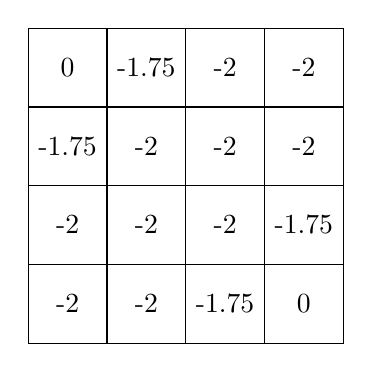
\begin{tikzpicture}
        % Define numbers for each cell
        \def\Numbers{{{"0","-1.75","-2","-2"},{"-1.75","-2","-2","-2"},{"-2","-2","-2","-1.75"},{"-2","-2","-1.75","0"}}}
        % Draw the grid
        \foreach \x in {0,...,3} {
            \foreach \y in {0,...,3} {
                % Draw each cell
                \draw (\x,3-\y) rectangle ++(1,1);
                % Place the number in the cell
                \node at (\x+0.5,3.5-\y) {\pgfmathparse{\Numbers[\y][\x]}\pgfmathresult};
            }
        }
        \end{tikzpicture}
\end{center}\par 
%==================================================================================================
\end{document}